\documentclass{standalone}

\usepackage[OT1]{fontenc}
\renewcommand*\familydefault{\sfdefault}
\usepackage{helvet,sfmath}
\usepackage{siunitx}

\usepackage{tikz}
\usetikzlibrary{arrows,calc,patterns}
\usepackage{tikz,tkz-euclide}


\definecolor{BlueDefault}{rgb}{0.2,0.2,0.7}

\begin{document}

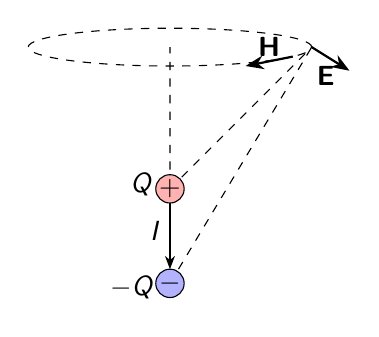
\begin{tikzpicture}[scale=0.6]
    %% Electromagnetic fields
    \draw[dashed]
    (0,1) to (3,4)
    (0,-1) to (3,4)
    (0,0) to (0,4)
    ;
    \draw[thick, -Stealth] (3,4) to (3.8,3.5);
    \draw[dashed] (0,4) ellipse (3 and 0.4);
    \draw[thick, -Stealth] (2.6,3.8) to (1.6,3.6);
    \draw 
    (3.3,3.4) node{\(\mathbf{E}\)}
    (2.1,4) node{\(\mathbf{H}\)}
    ;
    %% Dipole  
    \draw[-Stealth] (0,0.7) to (0,-0.7);
    \draw[fill = red!30] (0,1) circle(0.3);
    \draw[fill = blue!30] (0,-1) circle(0.3);
    \draw
    (0,1) node{\(+\)}
    (0,-1) node{\(-\)}
    (-0.3,0.1) node{\(I\)}
    (-0.6,1.1) node{\(Q\)}
    (-0.8,-1.1) node{\(-Q\)}
    ;
    
\end{tikzpicture}    

\end{document}